\documentclass{article}
\usepackage[margin=30mm]{geometry}
\usepackage[comma]{natbib}
\usepackage{todonotes}
\usepackage[toc,page]{appendix}
\usepackage{pdfpages}
\usepackage{graphicx}
\bibliographystyle{agsm}

\begin{document}
\title{Using Facial Recognition to gather Social Media Intelligence}
\author{Jack Neilson}
\maketitle
\newpage
\section{Literature Review}
\subsection{Background}
\subsubsection{SOCMINT}
Social media intelligence (SOCMINT) is an emergent field in intelligence gathering where data is gathered from social media profiles. Massive amounts of data are added to social media services every day \citep{socmintoverview}, much of it personal, making social media sites a potentially valuable resource when gathering information about groups or individuals \citep{gchqmasssurveillance}. Social networks have also been used as a means of communication between persons of interest to the security services, making mining intelligence from their profiles a high priority \citep{socmintoverview}\citep{policesocmint}.

After the 2011 riots in London that were organised in large part on social media, Her Majesty's Inspectorate of Constabulary stated that the police services were "insufficiently equipped" to effectively use SOCMINT in their response \citep{socmintpublicsafety} which suggests that social media intelligence sources may be woefully underutilised \citep{socmintoverview}. This is not to say that the value of SOCMINT is not realised however, as many intelligence agencies are investing in tools to effectively gather and analyse SOCMINT \citep{socmintpublicsafety} or are performing case studies in to potential uses \citep{bostonbombingcasestudy}.

While traditional human intelligence (HUMINT) focuses on building rapport and a foundation of trust in order to extract information from people of interest \citep{humintinterrogators}, users of social networking websites are much more likely to divulge personal information due to a misplaced senes of privacy \citep{socialmediacontent}. This makes SOCMINT attractive when attempting to gather data with little investment. The amount of data available to gather is vast in comparison to HUMINT sources \citep{socmintoverview}, making mass collection and analysis viable \citep{prismslides}. The nature of SOCMINT makes it easier to analyse than HUMINT, which relies on "tells" and small social cues \citep{humintinterrogators}.

\subsubsection{Uses of SOCMINT}
As previously stated, SOCMINT has seen some emergent use particularly in the security services. The Greek Ministry of Defence has developed a framework to identify individuals fitting certain psychiatric profiles from their social media accounts to allow for early identification of potential insider threats \citep{behaviourdetection}. By identifying factors that multiple intelligence agencies agree make a person more likely to pose an insider threat or negatively influence society (See appendix \ref{appendix:threatgraph}), they were able to map usage habits (intensity, content, popularity) to these factors to draw conclusions about clusters of users. So far, the research has been helpful in insider threat prevention, delinquent behaviour prediction and forensic analysis support.

\subsubsection{Facial Recognition}
Facial recognition is a much more mature area of research than SOCMINT with many examples of industry usage. Facebook uses facial recognition to automate "tagging" photos with the identity of the persons pictured \citep{facebookfacialrecog}, and large companies are now releasing datasets such as YouTube Faces \citep{faceregiondescriptors} in an effort to advance the field.

This is not to say that facial recognition is not without controversy however, as many privacy advocates have pointed out that accurate face regonition could infringe on their right to privacy \citep{gchqmasssurveillance}. David Wood and Lucas Introne have posed that accurate facial recognition could lead to increased levels of surveillance, with no way to "opt out" \citep{facialrecogpolitics}\citep{facialrecogsecurityvsprivacy}.

\subsubsection{Uses of Facial Recognition}
Facial recognition has many practical applications that are already being realised. As noted previously, Facebook uses facial recognition when "tagging" photos. This is presumably done to allow advertisers to more effectively target individual users - for example, a person identified in a photo with a barbeque may receive adverts for propane gas.

Facial recognition is also enjoying a heavy amount of attention from the security services due to it's use in identifying persons of interest. Case studies have been performed using images released to the public to ascertain how effective facial recognition is when looking for a specific person. In particular, Joshua Klontz and Anil Jain performed a case study using the images of the "Boston Bombers" against a set of test data \citep{bostonbombingcasestudy}. Their approach was successful in recognising one of the perpetrators from a picture taken from his social media account (See appendix \ref{appendix:bostonbomber}).

\subsubsection{Constrained vs Unconstrained}
While facial recognition software has come a long way, achieving accuracy rates of up to 99\% on small, consistent data sets \citep{facialrecogidentifyingpoi}, it is still in it's infancy when it comes to identifying people in "unconstrained" images. Images taken in the wild may have large variations in pose, facial occlusion and ambient lighting. This makes it difficult to identify facial features or markers (such as iris distinace, nasal distance, blemishes) which in turn has a negative impact on accuracy rates \citep{unconstrainedfacialrecogbenchmark}. When looking at applications of face recognition software with unconstrained datasets, matches are typically achieved when the test image has similar pose, facial occlusion and lighting as the sample image (See appendix \ref{appendix:bostonbomber}).

\todo{Do stuff here}
\subsection{Theory}
\subsubsection{Prior Work}

\subsection{Prior Knowledge Attacks}
\subsubsection{Social Engineering}
Social engineering in the context of information security refers to the ability of a person to gain access to information or control systems through a user or administrator, rather than through any technical oversight \citep{socialengineeringvulnerabilites}. It is a popular technique against "hardened" targets as technical prevention measures have proven to be ineffective \citep{advancedsocialengineering} making the human users and administrators the weakest link in the proverbial chain. In addition, it is difficult to train users in defenses against social engineering attacks. People believe they would not fall for such a trick despite research showing that humans perform poorly when attempting to detect deception \citep{advancedsocialengineering}\citep{socialengineeringvulnerabilites}. 

Social engineering using e-mail as a medium is ubiquitous \citep{socialengineeringvulnerabilites}. As a generel strategy, the person wishing to gather information will send one or more people an e-mail in hopes of a response (whether that be in the form of visiting a website, replying with their username or password, opening a file etc). Recent studies in realistic environments have had success rates of up to 23\% \citep{socialengineeringvulnerabilites} - this is especially worrying given that even 1 repsondant could compromise an entire company.

Examples of social engineering are not hard to find. In his book \textit{The Art of Deception} Kevin Mitnick describes a young Stanley Rifkin using social engineering to make the biggest bank heist of all time, stealing over 10,000,000 USD \citep{mitnick}. Social engineering attacks are certainly not difficult to perform - recently, a 13 your old child used social engineering to breach the private e-mail of the then-chief of the CIA, John Brennen \citep{cia13yearold}

\subsubsection{Spearphishing}
Spearphish attacks are a subsection of social engineering attacks wherein an attacker sends a malicous e-mail to a user that has been crafted using information that would make it seem authentic \citep{spearphishing}. For example, a normal social engineering attack using e-mail might send boilerplate messages to all personnel in a department to attempt to gain access to a network account. By contrast, a spearphish attack may use the names of specific people in the department, the location of the department, a spoofed e-mail header to make it seem as if the message came from within the department, and so on.

Social engineering attacks have proven to be effective at accessing sensitive information even when significant effort has been expended to secure it. A recent spearphishing campaign was conducted against 500 US military cadets - over 80\% clicked the link in the e-mail \citep{spearphishing}. Spearphish attacks are even more effective than "blind" phishing because of the additional information included in the e-mail which lulls the user in to a false sense of security (particularly when the information could be wrongfully considered "sensitive", for example including a manager's name and phone number).

Spearphish attacks in particular are difficult to mitigate against. They target the human element in information security making technological defenses insufficient \citep{spearphishing}. Education on spearphishing is not adequate to mitigate the potential threat either, as shown by William Pelgrin's exercise. He sent 10,000 New York State employees a phishing e-mail, and had a success rate of 15\% (that is, 15\% of users clicked the link in the e-mail then attempted to enter their passwords). The experiment was repeated after four months, with some success shown as the experiment had a success rate of 8\% \citep{spearphishingresults}. It must be remembered however that even a single successful spearphish attack could lead to a breach of information security.

\subsection{Intelligence Gathering}
\subsubsection{SOCMINT}
\subsubsection{HUMINT}
Human intelligence (HUMINT) pertains to the gathering of intelligence from individual human subjects. Information may be divulged non-consensually e.g. in the case of interrogation \citep{criminalvshumint}, or consensually in the case of clandestine information gathering \citep{clandestinehumint}. 

Non-consensual information gathering via interview or interrogation has only recently become a subject of study for the general public \citep{humintinterrogators}. 

Consensual information gathering sits in a much more grey area. Presenting yourself as somebody else may not be illegal depending on the circumstances, however it poses several moral questions. Clandestine intelligence gathering is still an extremely effective strategy, particularly when attempting to gather sensitive information which may be more heavily protected e.g. airgapped, firewalled \citep{clandestinehumint}. This makes it attractive during wartime or times of civil unrest \citep{humintni}\citep{humintcyberage}

Using a human intelligence approaches when gathering information has several downsides. It is a high risk strategy, as should a person be found out the consequences can be severe \citep{humintni}. The potential reward of sensitive information may be deemed to not be worth the risk. It goes without saying that HUMINT does not scale particularly well - it is a useful tool when attempting to extract information from a single person or small group, but it is much less useful when gathering information about larger groups. It relies on trust being built and may be ineffective when attempting to gather information from targets trained in tradecraft \citep{humintni}\citep{clandestinehumint}\citep{humintcyberage}.

\subsubsection{Individual vs Group Data}

\subsubsection{Quantity of Information}

\subsubsection{Accessibility of Data}

\subsubsection{Uses}
\todo{PRISM}

\subsubsection{Challenges and Constraints}





\subsection{Facial Recognition}
\subsubsection{Current Applications}

\subsubsection{State of the Art}	

\subsubsection{Challenges}

\subsubsection{Recent Advances}

\subsubsection{Unconstrained Facial Recognition}

\newpage
\bibliography{citations}

\newpage
\begin{appendices}
\section{Threat Graph}
\label{appendix:threatgraph}
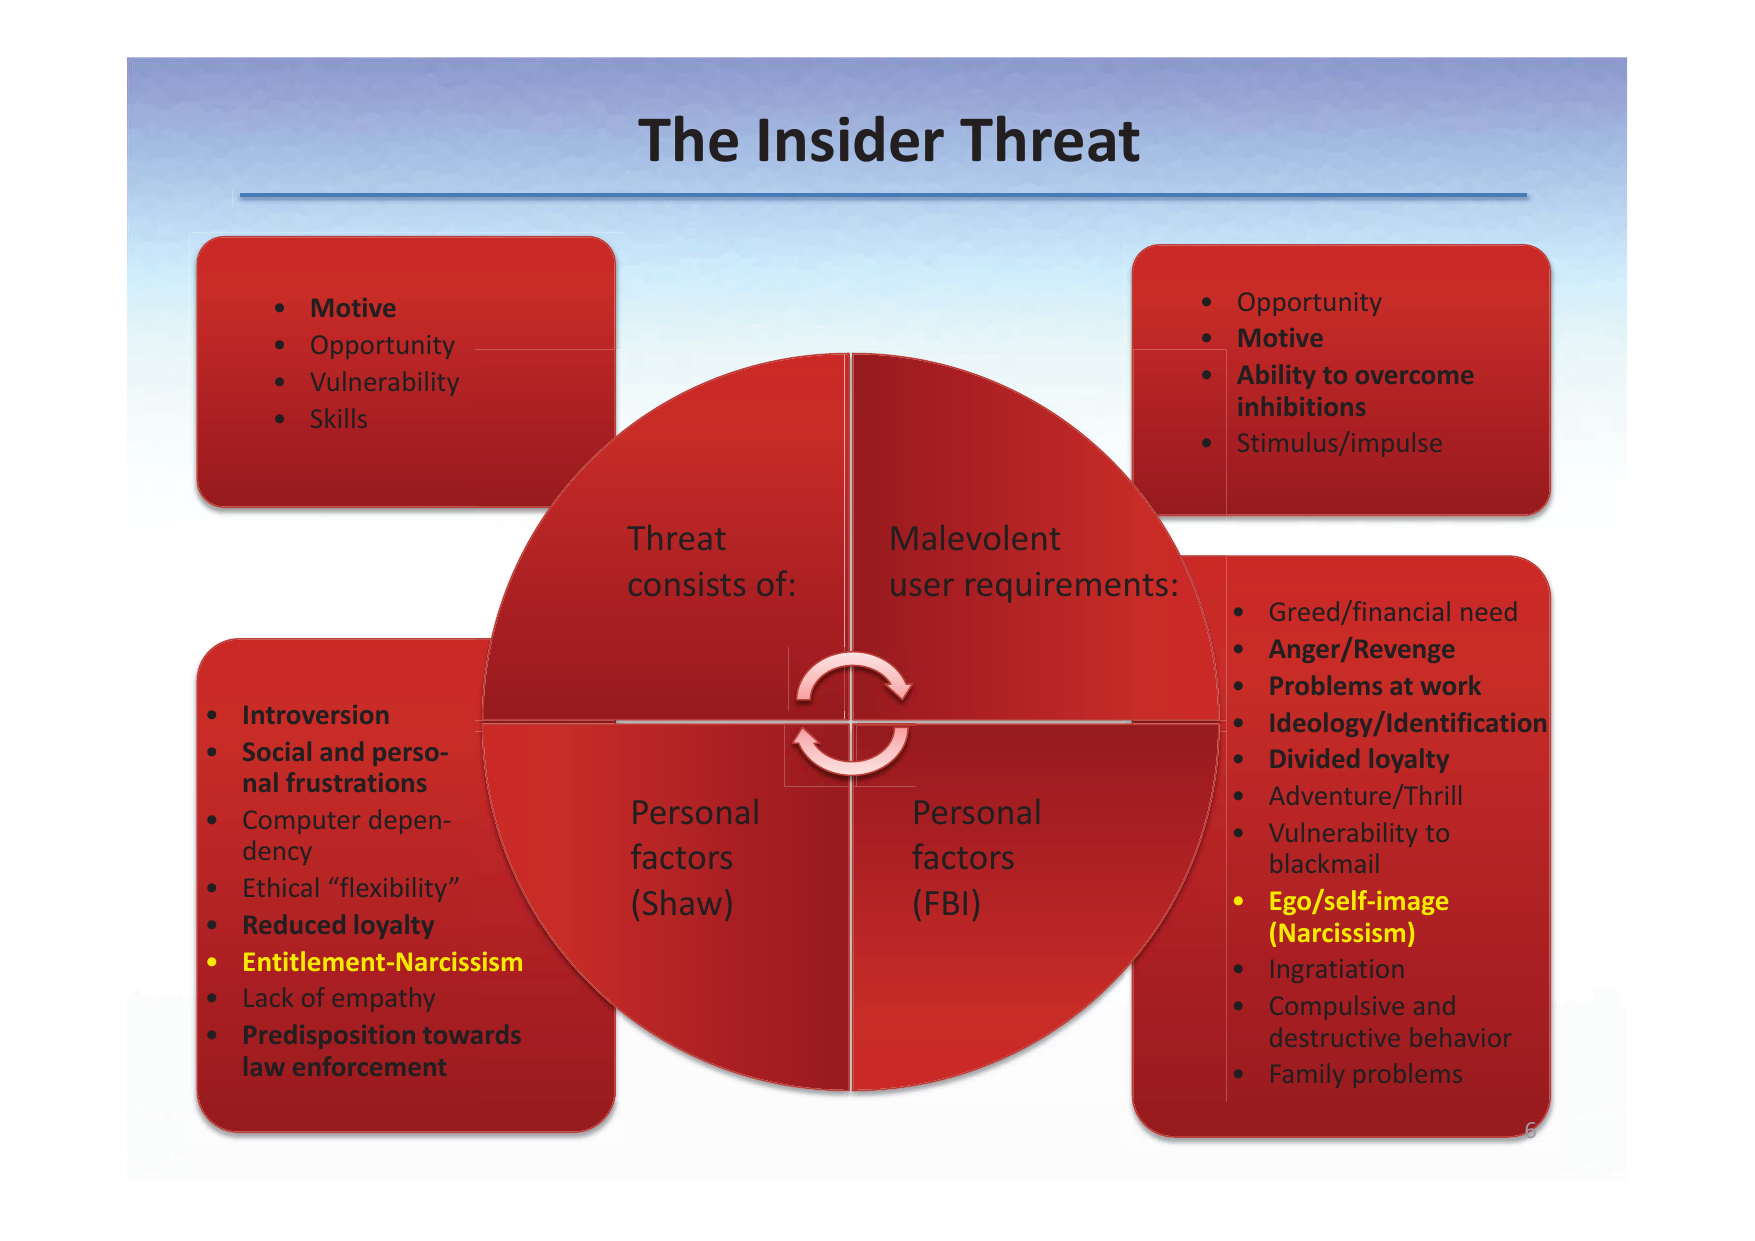
\includegraphics[width=\linewidth]{res/threat_graph.png}
Graph of insider threat factors \citep{behaviourdetection}.

\section{"Boston Bomber" Identification}
\label{appendix:bostonbomber}
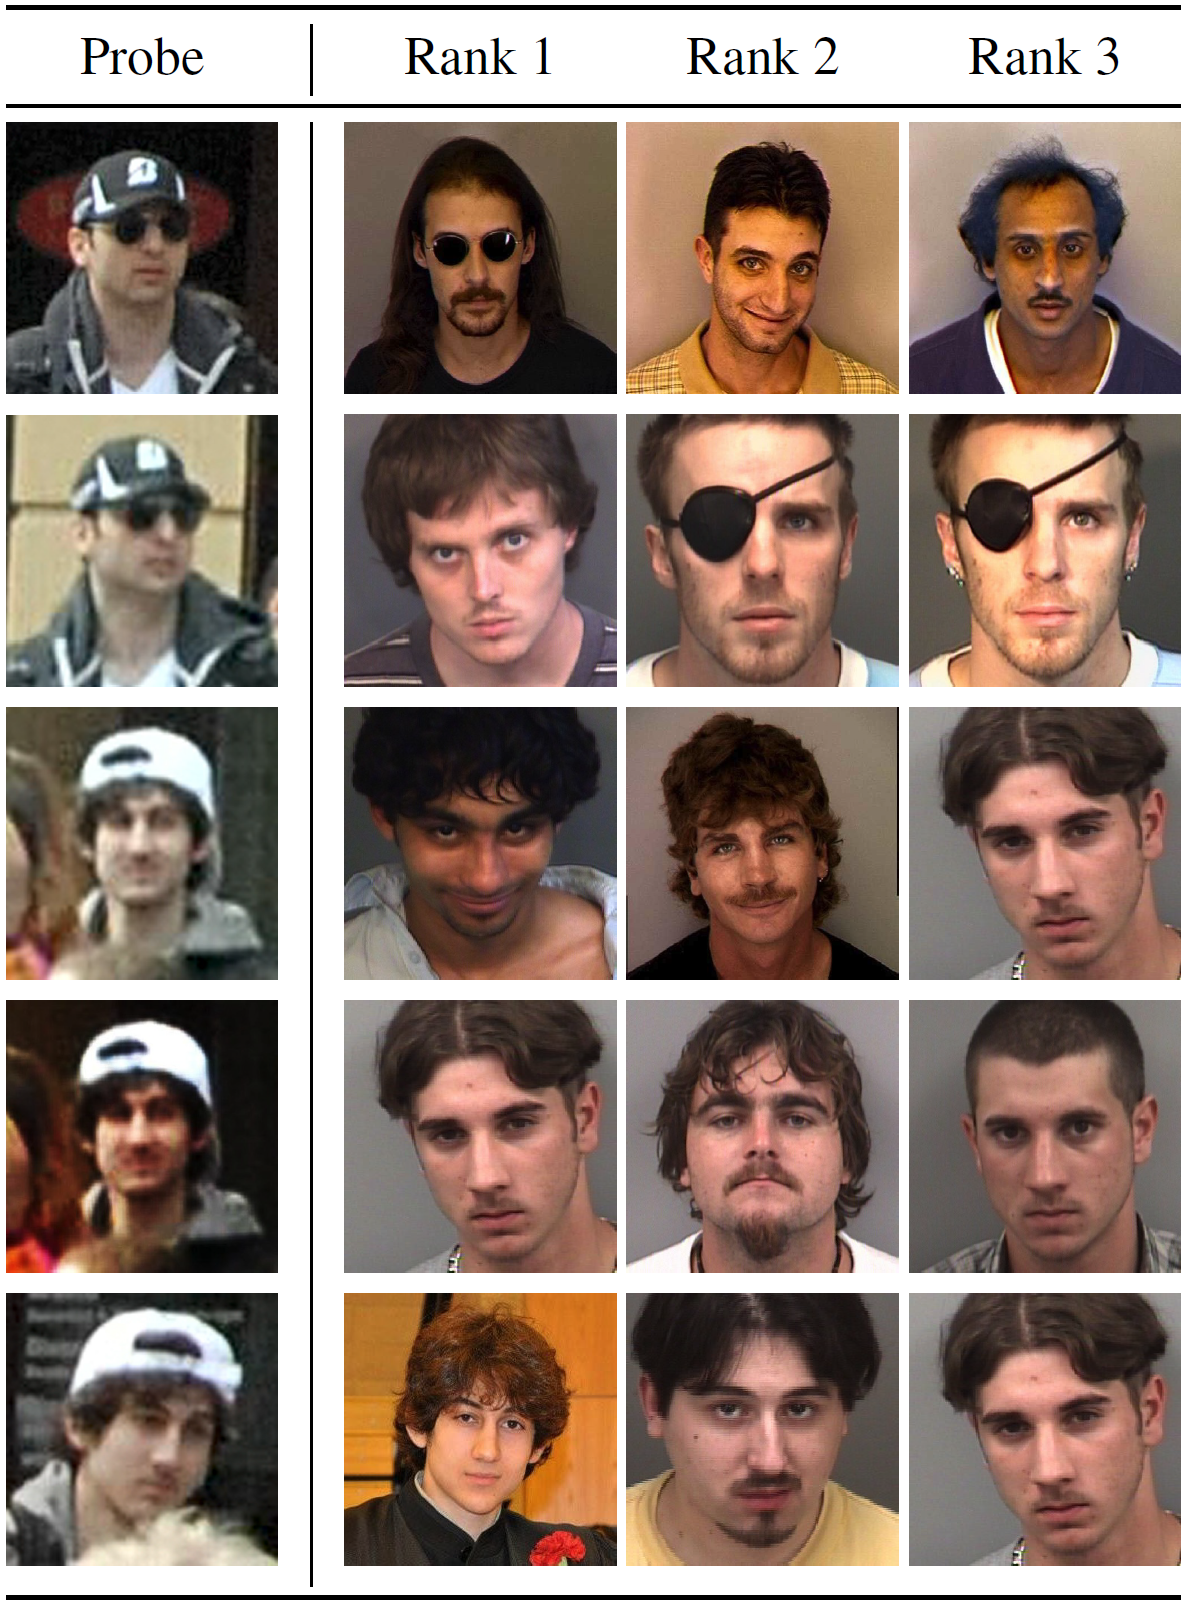
\includegraphics[width=\linewidth]{res/boston_bomber.png}
Table of potential matches, note the correct identification from the picture taken from social media with similar pose and lighting \citep{bostonbombingcasestudy}.

\end{appendices}

\newpage
\section{Methodology}
\subsection{Overview}
The software implemented will be in the form of a Python command line program, which allows users to specify an input image and data set to check it against. Additional identifying information such as name, date of birth etc. should also be utilised if given. The data sets the software references must come from social networking websites (or in the case of this proof of concept, a data set which is an accurate representation). 

As its output, the software must show the five most similar faces in the data set to allow for human verification. They should be presented with information that was gained from their social media profiles such as age, gender, name etc., as well as the similarity to the test image. In the case that the software is being ran headlessly, the results should be available in a file format which includes an image of the match and a representation of their social media profile.

\subsection{Functional Requirements}
\subsubsection{Face Recognition}
The software must implement a method of facial recognition, to rank a set of faces by similarity to a given test image. The test face must be extracted from the input image. The top 5 matches should be outputted, along with relevant identifying information.

\subsubsection{Social Media Integration}
The software must have the ability to use social networking websites as it's data set when comparing a test face. It would be desirable for the software to have the capability to use other identifying information alongside the test image to narrow the search space. Due to limited time and resources, test accounts may be used as a proof of concept.

\subsubsection{Headless}
The software should be able to function without a GUI, since the requirement of being able to use extremely large data sets may require deployment to a large server cluster or to a cloud.

\subsubsection{Multithreaded}
Where applicable, the software should make full use of parallelisation to increase its speed and resource utilisation. This is particularly important when working with large data sets.

\subsubsection{Deployment}
The software should make use of packaging systems, notably pip, to allow for easy deployment.

\subsubsection{Facial Recognition Libraries}
Due to time constrants, reimplementing facial recognition capabilities is not feasible. Therefore, the software should make use of already existing facial recognition libraries, in particular dlib or OpenCV.

\subsubsection{Language}
The software should be written in Python to allow for easy use of face recognition programs and rapid prototyping.

\subsubsection{Time Spent}
The software must be able to complete the above task in the same time or less than a human.

\subsubsection{Documentation}
The software should have at a minimum a man page and usage information. More documentation would be beneficial.

\subsubsection{Testing}
The software will be tested using a comination of \todo{Include final list of databases}

\subsection{Non-functional Requirements}
\subsubsection{Accuracy}
The software should have a \textit{relatively} high success rate when identifying a person from a social media collection. Note that typical facial reocgnition performance in unconstrained environments achieve a maximum success rate of ~30\%.

\subsubsection{Usefulness}
The information gained by using the software should help when crafting prior-knowledge attacks, increasing their effectiveness.

\subsubsection{Cross-Platform}
The software must be cross-platform to allow for easy deployment to servers or a cloud.

\subsubsection{Imprecision Tolerance}
The software should attempt a best guess when using an input image with less than ideal pose, facial occlusion or lighting. Inferior results when given a test image like this are acceptable to a degree.

\subsubsection{Usability}
The software is being developed for use by information security professionals in the form of a command line tool. This is ubiquitous in the industry, so no more than a cursory glance over the usage information should be needed to begin using the tool.


\section{Implementation}




\todo{Keep or remove this}
\section{Challenges}
\todo{Loading from mem rather than filesys}
\todo{Maximum loaded images}
\todo{Results from thread mutable object Deque}
\todo{Multiple workers for producing/consuming}




\section{Testing}
\section{Results}
\section{Evaluation}
\section{Conclusion}
\end{document}